\documentclass[a4paper]{report}

\usepackage[english]{babel}
\usepackage[utf8x]{inputenc}
\usepackage{amsmath}
\usepackage{graphicx}
\usepackage{xcolor}
\usepackage{listings}
\usepackage{hyperref}
\usepackage{amssymb}
\usepackage[square,sort,comma,numbers]{natbib}
\usepackage[colorinlistoftodos]{todonotes}
\bibliographystyle{ieeetr}

\lstdefinestyle{julia}{
  basicstyle=\scriptsize\ttfamily,
  breaklines=false,
  backgroundcolor=\color{gray!10},
}
\lstset{style=julia,
        emph={julia},
        emphstyle={\color{green}\bfseries}}


\title{Computational Methods for Parametrization of Polytopes}
\author{Steve Kelly}

%toc settings
\setcounter{tocdepth}{4}
\setcounter{secnumdepth}{4}

\begin{document}
\maketitle

%put table of contents
\tableofcontents
\clearpage 


\begin{abstract}
The combinatorial and geometric realization of polytopes are outlined in
mathematical and computational terminology. With these two representations in
hand, various parametric forms may be constructed using vertex locations, edge
angles, and symbolic values. We have implemented
software which represents polytopes in a way useful for combinatorial
inspection and solid modeling using the Julia programming language.
These packages have been published to GitHub and are accessible to
mathematical researchers around the world through the Julia package manager.
\end{abstract}


\chapter{Introduction}

Our objective is to develop a computational environment for the exploration
of parametric polytopes. Since a polytopes is assembled from simpler
primitives we will nessecarily develop these as well. Along our way, we
will hopefully see dichotomies and parallels in out mathemetical
classifications that reveal better structures.

To begin, we will define what it means in geometric and mathematical
terminology to be a polytope. We will seek to apply this type definition
in a way that is useful to both a programmer and a mathematician.
Such challenges in application are well known in
the Human-Computer Interaction (HCI) field. \cite{Tognazzini_1993}
How ever we approach this not an issue in the genre of the media,
but a strucutral one. As such, our media is computer code and we
will illustrate that the foundations in lamda calculus and
type theory are sufficient for our representations.

Finally we will demonstrate the preliminaries of our system. 

\todo{develop as body progresses}





\chapter{Mathematical Definitions}

In this section we will develop a mathematical perspective of our problem
such that we can focus clearly on the computational aspects in the following
sections. We are interested in parameterizing polytopes for
mathematical exploration. A polytope is geometrically realizable graph composed
of flat faces. Using the operations of union, intersection, and difference we
may say that a polytope of dimensionality N may be constructed using
hyperplanes of dimensionality N-1.
However the graph and hyperplane constructions are somewhat
distinct, and we will begin to see these representations
side by side as we move to a type framework.
For our purposes we will be concerned with polytopes which form closed solids.

To begin, we will outline how solids may be constructed using hyperplanes.

\section{Closed Spaces}

A "closed" space means a subset of something that contains all points in it's
boundary, including the bondary. An "open" set conversely will not include
the boundary, but everything inside.
We sometimes use brackets to aid the representation of sets on a number line
for example: (1,2) for an open set and
[1,2] for a closed set. The quantity of the objects contained in our sets
will vary depending on the numeric domain we choose.
For example if we are using integers we have no
elements in the open set and 2 in the closed set. If it is in rationals we
have 1/2 included, and in the reals we have infinite points! What we have
constructed on the number line can also be thought of as open
and closed intervals.

In multiple dimensions this is more interesting since we may construct
various, rather arbitrary, geometries to make a closed space.
One common example is a hyperplane. A hyperplane is simply a generalization
of the a plane into arbitrary dimensions, with the property it is
of dimensionality N-1. For example if we are in 2D space, our hyperplane
is a line since it partitions our space into two parts. Likewise in 3D
space this is a plane. If we define a hyperplane functionally using vector
notation we can extract some interesting properties.
For simplicity in this example let us assume we have a hyperplane which
cuts through the origin.
If we let 
$\vec{x}$ be an arbitrary point in $N$ dimensional space,
and $\vec{a}$ be the slopes of each axis, then one functional construction is
simply the dot product, $dot(\vec{a},\vec{x})$. If x is on the hyperplane
the function will be equal to zero. If it is not zero,
then we may determine which side of the partition the point lies on.
We notice that the hyperplane cuts space, but does not create a closed
subspace. Likewise the dot product definition gives us a measure of
area and we might rather prefer the shortest distance between the point
and the hyperplane. What we are after is what is known as a solid, and
we would like to do such using functions that return information useful
for computation.

\section{Solids and Orientation}

Before we define a polyhedra, we must introduce a few notions. These are
solids and orientation. Solids have been studied since
antiquity and for our purposes we will define them as constructions in
three dimensional space with finite volume.
For example, a plane which partitions space is not a solid
since either partition is unbounded, however the intersection of planes
could form a solid.

Orientation is a parallel concept which allows us to specify how geometric
objects contain space. As an example, let us go back to our partition of
space with a plane. If we are on our way to construct a solid, it is
neccessary to choose the one part to keep and the other to discard. This is
the purpose of orientation. In the case of the plane, this follows from the
definition, $ax+by+cz+d=0$. More lucidly, lets look at the signed distance
of a point from the plane, computed as:
\begin{equation}
D = \frac{ax+by+cz+d}{\sqrt{a^2+b^2+c^2}}
\end{equation}
For simplicity, let's look at a plane parallel to the X and Y axes passing
through z = 1. Thus $a$ and $b$ are set to 0, $c$ set to 1, and
$d=-1$
Simplifying our formulation we have:
\begin{equation}
$$ D = 0x+0y+z-1 = z-1$$
\end{equation}
At $z=1$ we see we are on the plane, however at $z=0$ and $z=2$ we get -1 and 1
respectively. The sign of the distance is our indicator of orientation. We can
choose an arbitrary convention as to which partition we will count, but akin
to the "right hand rule" in physics, the normals of the partition must point
outwards. In the case of the plane the normal is the vector $(a,b,c)$, which
in our realization is the upwards vector $(0,0,1)$. Since the convention is
such that the normals point outward, the partition we would consider in a
solid is all points \emph{in the opposite direction of the normal}.
Also to note is the importance of sign in our distance function. We can exploit
this behavior to indicate containment when performing logical operations on
spatial partitions. We have chosen this convention for this paper due to
it's ubiquity in computation frameworks.


\section{Distance Field Representations of Solids}

Implicit functional representation (FRep) in computation centers around a signed, real-value
function where the boundary is defined as $f(...) = 0$.
In $\mathbb{R}3$ this looks like $f(x,y,z) = 0$. For modeling purposes we must add the
additional constraint that the function evaluates to a negative inside the
boundary. Further more the magnitude of the return value must correspond to
the minimum distance between the point and the boundary.\cite{Olah_2011}
A sketch of this behavior in one dimension
can be seen in Figure \ref{fig:implicit-sketch}.

\begin{figure}[h!]
  \centering
    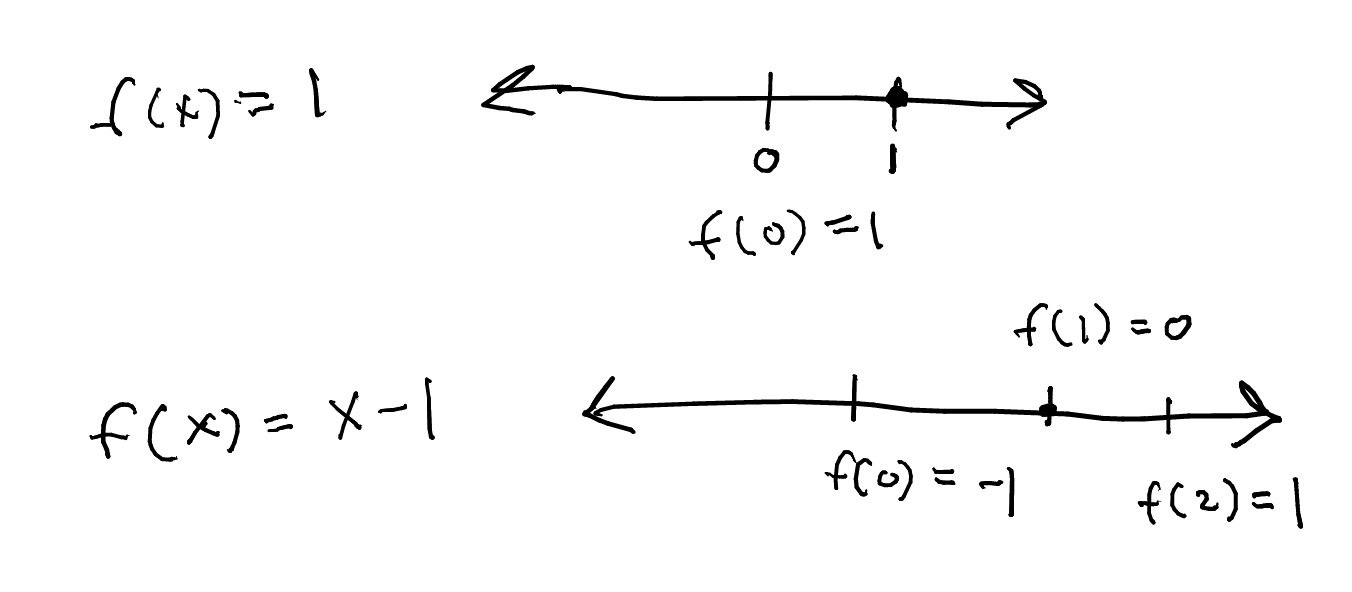
\includegraphics[width=0.75\textwidth]{img/implicit_sketch.png}
  \caption{Number line illustrating the construction of an implicit signed function}
  \label{fig:implicit-sketch}
\end{figure}

Researchers at MIT have taken these principles to constrain
geometric features to ensure a part can be manufactured.\cite{Shugrina_Shamir_Matusik_2015}
They call their system ``FabForms" and shows how functional representations
can easily accept constraints.

More importantly, functional representations can naturally deal with affine
transforms. \cite{Henderson_2002} Given some transform associated with a
FRep, one simply applies the inverse transform to check membership.

\section{Logical operations on Distance Fields}


One can also compose functional representations with set operations. 
Below are basic set operations defined for these functions:

\begin{equation*}
\cap : \mathtt{min}(f_1,f_2) \\
\end{equation*}
\begin{equation*}
\cup : \mathtt{max}(f_1,f_2) \\
\end{equation*}
\begin{equation*}
\neg : -\mathtt{f}_1
\end{equation*}

It follows that the ``difference"
of $f_1$ and $f_2$ is the intersection of $f_1$ with the negation of $f_2$,
$\mathtt{max}(f_1,-f_2)$.
The mathematical analyst might have trouble with these formulations because
such operations
create discontinuities.


\subsection{Rvachev Functions}

In the 1960's Vladimir Rvachev produced a method for handling the "inverse
problem of analytic geometry". His theory consists of functions which provide a
link between logical and set operations in geometric modeling and analytic
geometry.\cite{shapiro1991theory} While attempting to solve boundary value problems,
Rvachev formulated an equation of a square as
\begin{equation*}
a^2 + b^2 − x^2 − y^2 + \sqrt[]{( a^2 − x^2 )^2 +( b^2 − y^2 )^2} =0
\end{equation*}

Implicitly, the sides of a square can be defined as $x= +/- a$ and $y= +/- b$.
The union of these two is a square. By reducing the formulation of the square
we can generalize an expression for the union between two functions.
\begin{equation*}
\cup : f_1 + f_2 + \sqrt[]{f_1^2 +f_2^2} =0
\end{equation*}

Likewise we can see that intersections and negations can be formed for logical
completion.
\begin{equation*}
\cap : f_1 + f_2 - \sqrt[]{f_1^2 +f_2^2} =0 \\
\end{equation*}
\begin{equation*}
\neg : -f_1
\end{equation*}

These formulations can be modified for $C^m$ continuity for any $m$.
\todo{show this construction, it isn't obvious}
\cite{shapiro2007semi} In addition Pasko, et. al. have shown that Rvachev
functions can serve to replace a geometry kernel by creating logical
predicates. \cite{pasko1995function} Their research also establishes the
grounds for user interfaces and environment description. For this work a
practical implementation will most likely leverage their insights.
Rvachev and Shapiro have also shown that using the POLE-PLAST and SAGE
systems a user can generate complex semi-analytic geometry
as well.\cite{rvachev2000completeness} 

While a functional representation for geometry is mathematically enticing on
its own, the power it gives for numerical analysis might be its greatest
virtue. Numerical analysis justified the initial investigation by Rvachev
early on. A boundary value problem on a R-Function-predicate domain allows
for analysis without construction of a discrete mesh.\cite{rvachev2000completeness}

One of the most general expositions in the English language of R-Functions
applied to BVPs is
Vadim Shapiro's``Semi-Analytic Geometry with R-Functions". \cite{shapiro2007semi}
Unfortunately, no monographs about R-Functions exist in the English literature.
Most literature is in Russian, however many articles presenting applied
problems using the R-Function Method. \cite{voron2010}

Such a system for analytic geometry can be developed further. In the context
of an Eulerian flow field, a distance field over a function that
generates partial derivatives could be a fast numerical computation method.


\subsection{Signed Distance Fields}

\todo{rewrite to be salient}

A signed distance field (SDF) is a uniform sampling of an implicit function,
or any oriented geometry. \todo{didn't introduce orientation, winding order, etc...}
Below
we can see this in action over the definition of a circle.

\begin{lstlisting}
julia> f(x,y) = sqrt(x^2+y^2) - 1
f (generic function with 1 method)

julia> v = Array{Float64,2}(5,5) # construct a 2D 5x5 array of Float64

julia> for x = 0:4, y = 0:4
           v[x+1,y+1] = f(x,y)
       end

julia> v
5x5 Array{Float64,2}:
 -1.0  0.0       1.0      2.0      3.0    
  0.0  0.414214  1.23607  2.16228  3.12311
  1.0  1.23607   1.82843  2.60555  3.47214
  2.0  2.16228   2.60555  3.24264  4.0    
  3.0  3.12311   3.47214  4.0      4.65685
\end{lstlisting}

The results of \texttt{v} might be confusing since the matrix is oriented with
the origin in the top left corner. At coordinate $(0,0)$, or entry \texttt{v[1,1]},
we see that \texttt{f} is
equal to \texttt{-1}. Likewise we can see $(0,1)$ and $(1,0)$ are points on
the boundary since the value is \texttt{0} and everywhere else is positive.

Distance fields are interesting since they provide an intermediate representation
between functional space and discrete-geometric space. However they are
a very memory hungry data structure. Pixar has published OpenVDB which helps
work around these concerns, but such compression can be lossy.\cite{OpenVDB}
With the advent of shader pipelines for GPUs, distance fields have become
more popular. Valve has used SDFs with great success for generating smooth
text.text renders. \cite{Green_2007}
Many algorithms for generating polyhedra from an SDF
exist. The most common are Marching Tetrahedra, Marching Cubes,
and Dual Contours.\cite{Muller_Wehle_1997}\cite{Newman_Yi_2006}\cite{Cook_Hourvitz}

\todo{Talk about vert and frag shaders.}

Andreas Bærentzen and Henrik Aanæs published methods on the inverse
problem of converting a mesh to a signed distance fields.\cite{Baerentzen_Aanaes}
DiFi was introduced in 2004, which demonstrates an algorithm for creating
SDFs on multiple types of geometry \cite{Sud_Otaduy_Manocha_2004}.
\todo{Need to re-read this paper}

Many necessary algorithms in path planning for digital manufacturing tools
fall out of distance fields. For example, offsetting simply becomes
an addition or subtraction over the SDF. Computing the medial axis becomes
a scan for inflection points. Many path planners need to simplify polygon
representations as to not generate move less than the resolution of the machine.
Assuming the machine uses a Cartesian system, a SDF can correspond perfectly
to the lowest available resolution of the machine.
Likewise as Stereolithographic 3D printers
begin to use digital mirror devices (commonly known as DLP or DMD)
, discrete representations of geometry will become more important in
digital manufacturing.

\cite{Pasko_Adzhiev_Comninos_2008}

\section{Simplices}

Recently a Simplex type was added to GeometryTypes. A Simplex is defined
as the minimum convex set containing the specified points. The initial
prototype is very simple yet works well. Below we can see a 0th and 1st order
simplex constructed in $\mathbb{R}2$ and $\mathbb{R}3$
\begin{lstlisting}
julia> using GeometryTypes

julia> Simplex(Point(1,2))
GeometryTypes.Simplex{1,FixedSizeArrays.Point{2,Int64}}((FixedSizeArrays.Point{2,Int64}((1,2)),))

julia> Simplex(Point(1,2,3), Point(4,5,6))
GeometryTypes.Simplex{2,FixedSizeArrays.Point{3,Int64}}((FixedSizeArrays.Point{3,Int64}((1,2,3)),FixedSizeArrays.Point{3,Int64}((4,5,6))))
\end{lstlisting}

This representation makes it possible to write code based on the order and
dimensionality of a simplex. Few algorithms have been developed around the
new Simplex type, and unfortunately it is not integrated as a lower-level
construct for the other types yet.

In addition I would like to add a Simplical Complex type.\footnote{\url{https://en.wikipedia.org/wiki/Simplicial_complex}}


\section{Polytope}

\subsection{Descrete Form}


\subsection{Continuous Form}


\chapter{Computational Definitions and Grammar}

\todo{Needs massive refactor and redux}

Programming languages are the grammar and syntax a computer presents to a user.
This project is fundamentally exploratory in nature and seeks to generate
understanding of geometric relationships using the intersection of
mathematical and computational rigor. 


The REPL (Read-Eval-Print-Loop) allows interactive
evaluation of Julia code. It is highly useful for exploration and testing of
ideas in the language.
Blocks starting with "\texttt{julia>}" represent input and the preceding
line represents output of the evaluated line.

\subsection{History}
Julia is a programming language first released in early 2012 by a group of
developers from MIT. The language targets technical computing by providing a
dynamic type system with near-native code performance. This is accomplished by
using three concepts: a Just-In-Time (JIT) compiler to target the LLVM framework,
a multiple dispatch system, and code specialization.\cite{bezanson2012julia}
\cite{Bezanson_Edelman_Karpinski_Shah_2014}
The syntactical style is similar to MATLAB and Python.
The language implementation and many libraries are available under the
permissive MIT license.\footnote{\url{http://opensource.org/licenses/MIT}}

Benchmarks have shown the language can consistently perform within a factor of
two of native C and FORTRAN code.\footnote{\url{http://julialang.org/benchmarks}}
This is enticing for a solid modeling application and for numerical analysis,
as the code abstraction can grow organically without performance penalty.
In fact, the authors of Julia call this balance a solution to the 
``two language problem". The problem is encountered when abstraction in a
high-level language will disproportionately affect performance unless
implemented in a low-level language. In the next sections we will compare
the expressibility and performance to other languages.

\subsection{Comparisons}

Many languages are as fast as Julia but sacrifice expressibility.
In Figure \ref{fig:juliabench} we can see some comparisons to other programming
languages. This was developed by the Julia core team, and illustrates that
Julia is highly competitive in performance. Again, these results stem from
the compiler and language design. In Figure \ref{fig:juliaexpr} we can see
these results normalized against code length. The Julia code is quite short,
yet consistently achieves good performance.
Much of this comes down to the innovated type and function system.\cite{Chen2014} We will
discuss these more in depth later.

\begin{figure}[h!]
  \centering
    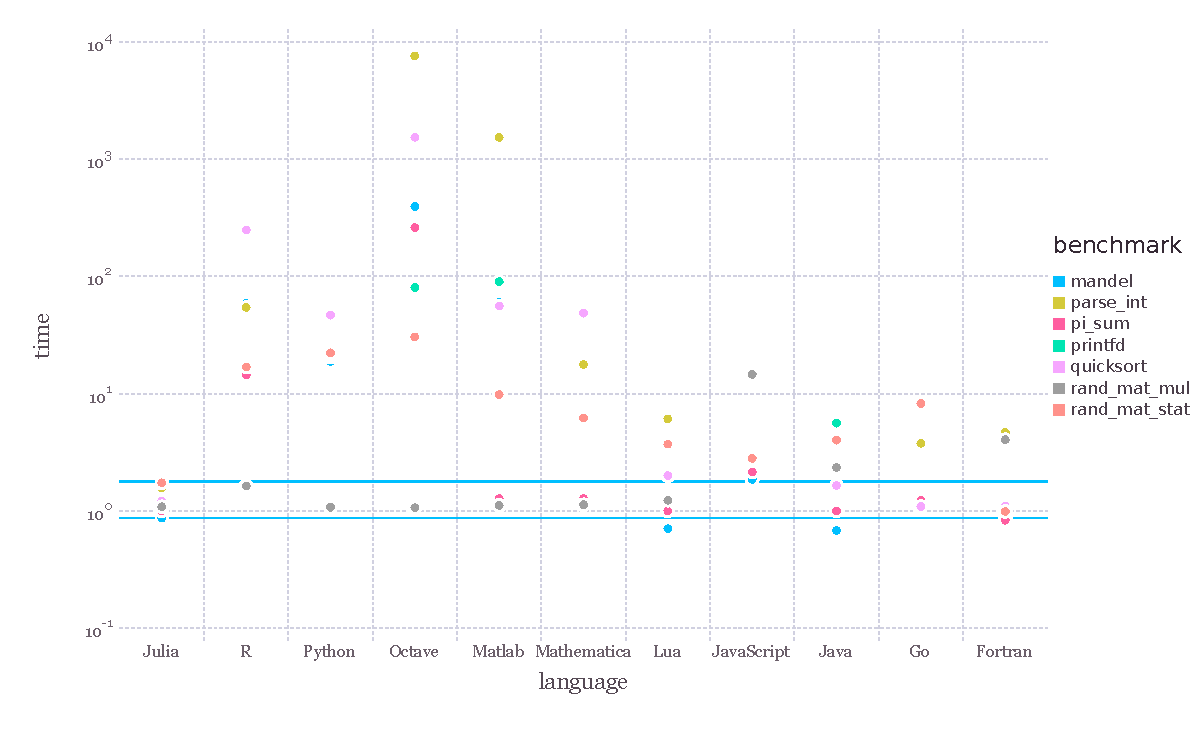
\includegraphics[width=1.0\textwidth]{img/juliabench.pdf}
  \caption{A comparison of programming languages and performance.}
  \label{fig:juliabench}
\end{figure}

\begin{figure}[h!]
  \centering
    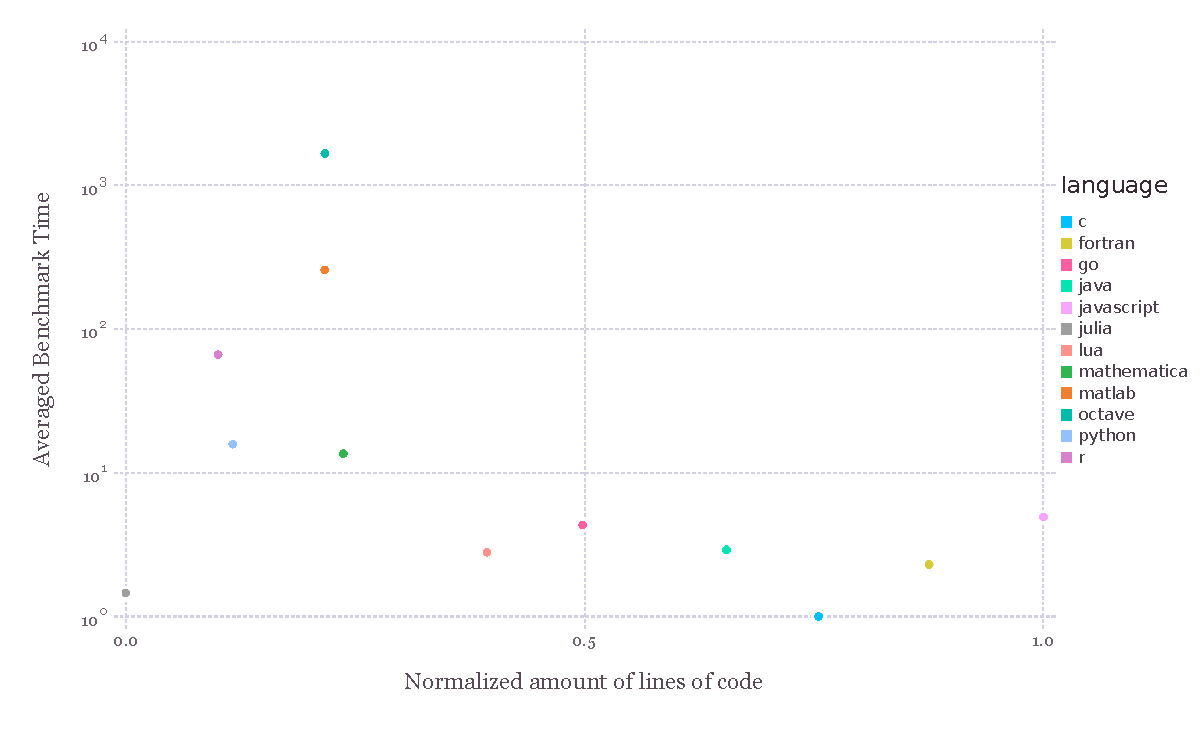
\includegraphics[width=1.0\textwidth]{img/expressability.pdf}
  \caption{The results in Figure \ref{fig:juliabench} normalized for code length. (Courtesy of Simon Danish)}
  \label{fig:juliaexpr}
\end{figure}


In 1972 Alan Kay introduced the terms
"class" and "object", to describe a coupling of data and functionality.\footnote{\url{http://gagne.homedns.org/~tgagne/contrib/EarlyHistoryST.html}}
An object is simply and implementation of a class. Computer Scientists
call this "Object Oriented Programming" (OOP).
Languages such as C++, Java, and Python all subscribe to this paradigm.
In Python this looks like the following:
\begin{lstlisting}
class Foo:
    foo1
    foo2
    def add_to_foo1(self, x):
        self.foo1 += x
\end{lstlisting}

This system positively enables specialization of functionality, but due
to the coupling of data with functions it becomes a challenge to extend
functionality. Languages for scientific computing generally avoid the
"traditional" notions
of OOP. In Table \ref{tab:types} we can see a
comparison of type systems used in scientific computing languages. In the next
few sections the implications of multiple dispatch and the relation to OOP
will be developed further.


\begin{figure}[h!]
  \centering
    \caption{A comparison of functions, typing, and dispatch.}
    \begin{tabular}{ l | l l l}
    Language & Type system & Generic functions & Parametric types \\
    \hline
    Julia & dynamic & default & yes \\
    Common Lisp & dynamic & opt-in & yes (but no dispatch) \\
    Dylan & dynamic & default & partial (no dispatch) \\
    Fortress & static & default & yes \\
    \end{tabular}
  \label{tab:types}
\end{figure}


\subsection{Functions}
Julia is an experiment in language design. Much of the advancement
revolves around the representation of data and the execution of functions.
The language is optionally typed, which means function specialization on types
is inferred. We will use it See below:
\begin{lstlisting}
julia> increment(x) = x + 1
increment (generic function with 1 method)

julia> increment(1)
2

julia> increment(1.0)
2.0
\end{lstlisting}
the \texttt{increment} function was defined for any \texttt{x} value. When the
\texttt{1}, an
integer type was passed as an argument, an integer was returned. Likewise
when a floating point, \texttt{1.0} was passed, the floating point
\texttt{2.0} was returned.

Let's see what happens when we try a string:
\begin{lstlisting}
julia> increment("a")
ERROR: MethodError: `+` has no method matching +(::ASCIIString, ::Int64)
Closest candidates are:
  +(::Any, ::Any, ::Any, ::Any...)
  +(::Int64, ::Int64)
  +(::Complex{Bool}, ::Real)
  ...
 in increment at none:1
\end{lstlisting}

The problem is that the \texttt{+} function is not implemented between the
\texttt{ASCIIString} and \texttt{Int64} types.
We need to either implement a \texttt{+} function
which might be ambiguous, or specialize the function for \texttt{ASCIIString}.
A specific implementation is preferrable in this case:
\begin{lstlisting}
julia> function increment(x::ASCIIString)
           ASCIIString([increment(c) for c in x])
       end
increment (generic function with 2 methods)
\end{lstlisting}
The line \texttt{x::ASCIIString} is called a ``type annotation" and
states that \texttt{x} must be a subtype
of \texttt{ASCIIString}. This allows one to control dispatch of functions,
since Julia will default to the \emph{most specific implementation}.
Since\texttt{ASCIIString} is a series of 8 bit characters, we can iterate over the
string and increment each character individually. The \texttt{[]} indicates we are
constructing an array of characters to pass to be passed to the \texttt{ASCIIString}
type constructor. Now we see our example works:
\begin{lstlisting}
julia> increment("abc")
"bcd"
\end{lstlisting}

What was demonstrated here is the concepts of specialization and multiple
dispatch, both are highly coupled topics.
Each function call in Julia is specialized for types if possible.
This means the author only has to write a few sufficently abstract
implementations of functions. If special cases occur multiple functions
with different arity or type signatures can be implmented. Explicitly
this is called multiple dispatch. In practice by the user this looks like
abstracted or generic code.
To the computer, this means choosing the most specific, and
thus performant method. Let's go back to the integer and floating point
example. Below is the LLVM assembly generated for each method:
\begin{lstlisting}
julia> @code_llvm increment(1)

define i64 @julia_increment_21458(i64) { // <return type> <function name>(<arg type>)
top:
  %1 = add i64 %0, 1
  ret i64 %1 // return <return type> <return id>
}

julia> @code_llvm increment(1.0)

define double @julia_increment_21466(double) {
top:
  %1 = fadd double %0, 1.000000e+00
  ret double %1
}
\end{lstlisting}

Note I have annotated the LLVM code so this is understandable. 
The only real similarity is the line count. Each one of these functions are generated by the
Julia compiler at run time.

Many of the concepts used for performance also serve as methods for
expressability. In this case, multiple dispatch used by the compiler for
specialization of functions reveals it self as a way for the user to
specialize over many types.
Revealing the role in which this paradigm allows Julia to achieve high
performance is a matter to be developed in further sections.

\subsection{Types}

\subsubsection{Mutability and data packing}
Types and immutables are containers of data. The primary difference between
the two is the notion of "mutability". Types are mutabile, immutables are 
immutable. What does this mean? Let's break something first:
\begin{lstlisting}
julia> type FooIsMutable
           a
       end

julia> f = FooIsMutable(1)
FooIsMutable(1)

julia> f.a
1

julia> f.a = 2
2

julia> f.a
2

julia> immutable FooIsImmutable
           a
       end

julia> f = FooIsImmutable(1)
FooIsImmutable(1)

julia> f.a
1

julia> f.a = 2
ERROR: type FooIsImmutable is immutable
\end{lstlisting}

What just happened demonstrates the contract defined by mutability. Mutable
objects, which is an instance of a type (i.e. \texttt{f}), can have their fields
(i.e. \texttt{a}) changed. Immutables cannot. The immutable contract helps develop
a notion of functional purity. To the user this means immutables are defined
by their values. Practically this can be of great benefit to
the compiler. For example:
\begin{lstlisting}
julia> a = (1,2,3)
(1,2,3)

julia> b = typeof(a)
Tuple{Int64,Int64,Int64}

julia> isbits(b)
true

julia> a = ([1],[2],[3])
([1],[2],[3])

julia> b = typeof(a)
Tuple{Array{Int64,1},Array{Int64,1},Array{Int64,1}}

julia> isbits(b)
false
\end{lstlisting}

\texttt{isbits} ask the question ``will this type be tightly packed in memory"? A
\texttt{Tuple} is a fixed-length set of linear, ordered, data. It has syntax for
construction with \texttt{()}. In computations we want our data be close together
for fast access. In modern times we call such data "cache friendly", or
"cache localized". Immutability helps us achieve this. Let's look that the
types inside the 3-tuples and see their \texttt{isbits} status:
\begin{lstlisting}
julia> isbits(Array{Int64,1})
false

julia> isbits(Int64)
true
\end{lstlisting}
Why is this the case? We see that \texttt{Int64} is bits, because it is literally
64 bits. In Julia a \texttt{bitstype} behaves similar to an immutable, and is identified
by value. \texttt{Array\{Int,64\}} is a mutable data type that can vary in size.
This means
the \texttt{Tuple} needs to store the arrays as references, in this case a
pointer. When iterating over a data set, such a ``pointer dereferences" (this is
jargon for accessing the data in memory pointed to by a pointer), can be costly.
Modern CPUs accell when data is linearly packed and pointer-free. The
data can be brought into the CPU's memory cache once and computed without
shuffling between cache and RAM.

\subsubsection{Parameters}

\todo{need to demonstrate why this is HUGELY important for performance and expression}

\subsubsection{Macros and Generated Functions}
Julia is a descendant of the Lisp family of programming languages. Lisp
is a portmanteau for "List Processing". The language was designed to address
the new notion of "types", specifically in application to Artificial
Intelligence (AI) problems.\cite{McCarthy_1966} The notion of an "S-Expression"
was introduced in McCarthy's seminal work. These statements use parenthesis
to denote functions and arguments. Below is an an example of S-Expressions
for addition and multiplication.

\begin{lstlisting}
> (+ 1 1)
2

> (* 3 4)
12
\end{lstlisting}

This syntax is noted for it's mathematical purity.
However it can be a syntactic difficulty for many.
Most of the current popular programming languages
use variants of ALGOL syntax, which is noted for being more readable.
\cite{Hoare}
Julia also uses ALGOL syntax, but is lowered to S-Expressions. This enables
many of the mathematically pure relations we seek to achieve.
In addition S-Expressions are highly conducive to source transforms.
This develops a notion of "Homoiconicity", where the representation of
program structure is similar to the syntax. In Julia we use this property
to make "macros" which enable source code to be transformed based on
structure before compilation.

Generated functions perform a similar function as macros, but at the function
level. They enable source code to be procedurally generated based on types.
Surveys of Computer Science literature show that such a concept is new.
\todo{More on generated functions. Not sure if they should even be mentioned
since they are usually unnecessary}

\todo{More articulate like Graydon Hoare: \url{http://graydon2.dreamwidth.org/189377.html}}

\subsection{Example}

\cite{Shamos_1999}



\chapter{Implementation}

In this section we will begin to outline the implementation of
various forms of parametric polytopes.

\section{Survey of Available Packages}

In chapter 3 we outlined the rationale for using Julia for mathematical
computer programming. An additional impetus was the familiarity of the
geometry packages. There will be various references to these and they
are outlined below so the reader may become familiar with the utilities
available.

\subsection{GeometryTypes.jl}

GeometryTypes.jl provides datatypes and basic operations for computational
geometry. This package began as a unification of types located in
HyperRectangles.jl, Meshes.jl, and GLAbstraction.jl. The initial
types were polygonal meshes and bounding boxes, but now encompasses
datatypes for solid modeling, data visualization, and
geographic information systems.
With the introduction
of this package the community made some initial progress on designing
types that can be used for computation on the CPU and GPU, however
GPU targets are rapidly evolving and the focus has shifted from geometric
operations to array operations. Much of
our basic combinatorial analysis operations and data types have be contributed
to this package.

\url{https://github.com/JuliaGeometry/GeometryTypes.jl}

\subsection{FileIO.jl and MeshIO.jl}

FileIO.jl is a package that unifies various file loaders that existed in
the Julia package ecosystem under one import. The purpose is to
allow users to simply call the \texttt{save} and \texttt{load}
functions with file
information inferred from file extensions, magic numbers, or data types.
MeshIO.jl is one such packge that provides file loaders for
polygonal mesh data. The file formats supported as of this writing include
obj, stl, ply, off, and 2dm. This package may be useful for importing
polytope data from other programs such as Blender or AutoCAD, or generating
large data sets.

It should be noted that Julia has a \texttt{serialize} function, which will
save a datatype in full fidelity and in compact binary. Since Julia is
yet to reach a 1.0 release, this function is considered unstable. Once
\texttt{serialize} is stable, it will be the preferred method of saving
data sets to the computers storage drive.

\url{https://github.com/JuliaIO/FileIO.jl}

\url{https://github.com/JuliaIO/MeshIO.jl}

\subsection{Meshing.jl}

Meshing.jl provides algorithims for converting signed distance field
data into polytopes. The two algorithms currently provided are
the Marching Cubes (MC) and Marching Tetrahedra (MT) algorithms. For this project
we added the Marching Cubes algorithm which is twice as fast as the
Marching Tetrahedra algorithm. The import difference between the two is
performance and manifold mesh generation. The MT algorithm generates manifold
meshes, but generates more faces (costing memory) and is slower.
It is useful for generating
meshes from noisy data or applications where manifold meshes are required
such as finite element analysis and 3D printing. The Marching Cubes algorithm
is less costly for the computers resources, and is helpful for visualization
applications where user experience is important.

\url{https://github.com/JuliaGeometry/Meshing.jl}

\subsection{Meshes.jl}

Meshes.jl is currently a meta-package\footnote{Meta-package means
no code is contained in the package besides imports from others. It is
often used for stability purposes.} that imports elements on GeometryTypes.jl,
FileIO.jl, and Meshing.jl. It is one of the older packages in the
Julia package ecosystem and was an early center of collaboration before
the scopes began to expand. Releases before Meshes.jl became a meta-package 
are maintained for insitutional users. The name space is held to
allow for a center for experimentation as stability in the base packages
becomes more neccesary.

\url{https://github.com/JuliaGeometry/Meshes.jl}

\subsection{ParametricPolyhedra.jl}

ParametricPolyhedra.jl is a package used for solving constraints on
triangular faces of a polyhedra. The intention of this package
is to allow polyhedra to be specified via angles and edge lengths.
It draws heavily from the resources available in GeometryTypes. Since
it uses algorithms to define the types and is some what domain
specific at this point, we opted to make it a seperate package.

\url{https://github.com/sjkelly/ParametricPolyhedra.jl}

\subsection{GeometricalPredicates.jl}

GeometricalPredicates.jl is a package that provides numerically
robust primitives and algorithms for computing incircle, circumcircle, and
intriangle calculations. The approach to numerical robustness is used by
the Illustric Simulation, and outlines in Volker Springel's paper
"Galiliean-invariant cosmological hydrodynamical simulations on a moving mesh"\cite{Springel_2010}.
The essence of the approach is to restrict values in 64 bit floating points
between 1 and 2 since the exponent component is constant. This allows
128 bit integers to be used for overflow calculations.

\url{https://github.com/JuliaGeometry/GeometricalPredicates.jl}

\section{GeometryTypes.jl Implementations}

\section{Simplex}

We began by implementing a Simplex type in GeometryTypes.jl,
defined as follows:

\begin{lstlisting}
"""
A `Simplex` is a generalization of an N-dimensional tetrahedra and can be thought
of as a minimal convex set containing the specified points.

* A 0-simplex is a point.
* A 1-simplex is a line segment.
* A 2-simplex is a triangle.
* A 3-simplex is a tetrahedron.

Note that this datatype is offset by one compared to the traditional
mathematical terminology. So a one-simplex is represented as `Simplex{2,T}`.
This is for a simpler implementation.

It applies to infinite dimensions. The sturucture of this type is designed
to allow embedding in higher-order spaces by parameterizing on `T`.
"""
immutable Simplex{N,T} <: AbstractSimplex{N,T}
    _::NTuple{N,T}
end
\end{lstlisting}

With the definition in GeometryTypes, we afford ourselves two notions of
dimensionality. Our first parameter \texttt{N} gives us the total dimensionality
of the simplex. We will notice that our convention is offset by positive one
compared to the mathematical terminology. This is due to Julia not allowing
arithmetic in type defintions. There are a few approaches to circumvent this
issue, but they either make the datatype larger or sacrifice strong
type inference.

The second parameter, \texttt{T} is the type of the points. We will see that
point may be symbolic in nature, or have their own dimensionality
expressed independent of \texttt{N}.
For example in Julia we
may
prefix a colon to an identifier and make it a symbolic value which is reflected
in the type information:

\begin{lstlisting}
julia> using GeometryTypes

julia> Simplex(:x,:y,:z)
GeometryTypes.Simplex{3,Symbol}((:x,:y,:z))
\end{lstlisting}

In this example we have created a 2-simplex with symbols \texttt{:x, :y, :z}.
\texttt{N} is 3, and \texttt{T} has become \texttt{Symbol}.
Symbolic representation will allow us to create simple combinatorial
analysis.
Likewise we can construct concrete types:

\begin{lstlisting}
julia> Simplex(Point(0,0,0), Point(1,1,1))
GeometryTypes.Simplex{2,FixedSizeArrays.Point{3,Int64}}((FixedSizeArrays.Point{3,Int64}((0,0,0)),FixedSizeArrays.Point{3,Int64}((1,1,1))))
\end{lstlisting}

This last example illustrates how \texttt{N} and \texttt{T} may give us
two notions of dimensionality in the Simplex.
Here we have constructed a line segment in 3D space. The Simplex is of
size two but the space it occupies is three dimensional. This way it acts
similar to a fixed size vector, but the type implies all points are on the
convex hull. Unfortunately it may also be possible to construct a Simplex
using points of dimension less than that of the Simplex, which would
not hold to our contract of linear independence.
More so we may also decompose its

Below is an example of a high performance implementation of Simplex decomosition:

\todo{update code example}


\section{HomogenousMesh Type}

Prior to this project, GeometryTypes primarily provides for Polygonal Mesh
type that is well tuned for operations on the CPU and GPU. It is defined
as follows:

\begin{lstlisting}
"""
The `HomogenousMesh` type describes a polygonal mesh that is useful for
computation on the CPU or on the GPU.
All vectors must have the same length or must be empty, besides the face vector
Type can be void or a value, this way we can create many combinations from this
one mesh type.
This is not perfect, but helps to reduce a type explosion (imagine defining
every attribute combination as a new type).
"""
immutable HomogenousMesh{VertT, FaceT, NormalT, TexCoordT, ColorT, AttribT, AttribIDT} <: AbstractMesh{VertT, FaceT}
    vertices            ::Vector{VertT}
    faces               ::Vector{FaceT}
    normals             ::Vector{NormalT}
    texturecoordinates  ::Vector{TexCoordT}
    color               ::ColorT
    attributes          ::AttribT
    attribute_id        ::Vector{AttribIDT}
end
\end{lstlisting}

The first thing to note is the provisions for attributes, colors, and textures.
These are used for mapping textures and/or colors to polygons via visualization
software such as
OpenGL. We do not need these in a rigourous mathematical
definition. Likewise, in a HomogenousMesh we structure the realization as
follows: 1. Insert all vertices of the mesh into \texttt{vertices} 2. Construct
faces of at least 3 indices referencing the points in \texttt{vertices}.

This gives us certain properties that are nice for computation. Primarily
this allows us to observe the combinatorial properties of the mesh by analyizing
the faces. In addition, this compacts the data representation of vertices
since shared vertices can be represented with a common face index. Affine
transforms only need to operate on the vertices, and if it is closed and
faces share many vertices this may be up to 3 times faster.

However the most important issue with this type is that it is not
parameterized as a Polytope, and simply as a polyhedral mesh.

\section{Polytope Type}

We implemented a Polytope to address some of the issues with the
\texttt{HomogenousMesh} type. It is defined as follows:

\begin{lstlisting}
"""
A `Polytope` is an `N` dimensional object with elements `T` of the same type.
For example typealias `Polygon` and `Polyhedron` exist for dimensions 2 and
3 respectively.
"""
type Polytope{N,T} <: AbstractPolytope{N,T}
    elements::Vector{T}
end
\end{lstlisting}

The supertype \texttt{AbstractPolytope} type is not implied in the mathematical
sense, but rather to allow more granular definitions as needed for different
computational challenges. The \texttt{Polytope} type is parameterized
by \texttt{N}, the order of the polytope. The following
aliases exist for Polytopes with specified values for \texttt{N}:

\begin{lstlisting}
"""
A `Polygon` is a `Polytope` realizable with only two dimensions.
Generally this will be composed of `Points` or `LineSegment`s.
"""
typealias Polygon{T} Polytope{2,T}

"""
A `Polyhedron` is a `Polytope` realizable with only three dimensions.
Generally this will be composed of `Face`s or two-simplices (`Simplex{3}`).
"""
typealias Polyhedron{T} Polytope{3,T}
\end{lstlisting}

The final parameter, \texttt{T}, is the type of the elements. This may
simplify many representations, and allow more liberty in Polyhedron
representation. For example, constructions of polygons are straight forward
and may be a \texttt{Vector} of \texttt{Symbol} or \texttt{Point}.
However a Polyhedron may be constructed from \texttt{Simplex} or
\texttt{Polygon}. In this way it behaves as a wrapper of a \texttt{Vector}
with special type information associated. Of course, non-sensical constructions
may be made, but with sufficiently parameterized functions they will not
be operable.

\subsubsection{Functions}

Along with defining a \texttt{Polytope} we have added calculations for
area, volume, centroids, and various decomposition functions.

\url{https://github.com/JuliaGeometry/GeometryTypes.jl/pull/27}


\subsection{Signed Distance Fields}

A signed distance field (SDF) is a uniform sampling of an implicit function.
It was implemented earlier as a 
Below
we can see this in action over the definition of a circle.

\begin{lstlisting}
julia> f(x,y) = sqrt(x^2+y^2) - 1
f (generic function with 1 method)

julia> v = Array{Float64,2}(5,5) # construct a 2D 5x5 array of Float64

julia> for x = 0:4, y = 0:4
           v[x+1,y+1] = f(x,y)
       end

julia> v
5x5 Array{Float64,2}:
 -1.0  0.0       1.0      2.0      3.0    
  0.0  0.414214  1.23607  2.16228  3.12311
  1.0  1.23607   1.82843  2.60555  3.47214
  2.0  2.16228   2.60555  3.24264  4.0    
  3.0  3.12311   3.47214  4.0      4.65685
\end{lstlisting}

The results of \texttt{v} might be confusing since the matrix is oriented with
the origin in the top left corner. At coordinate $(0,0)$, or entry \texttt{v[1,1]},
we see that \texttt{f} is
equal to \texttt{-1}. Likewise we can see $(0,1)$ and $(1,0)$ are points on
the boundary since the value is \texttt{0} and everywhere else is positive.

Distance fields are interesting since they provide an intermediate representation
between functional space and discrete-geometric space. However they are
a very memory hungry data structure. Pixar has published OpenVDB which helps
work around these concerns, but such compression can be lossy.\cite{OpenVDB}
With the advent of shader pipelines for GPUs, distance fields have become
more popular. Valve has used SDFs with great success for generating smooth
text.text renders. \cite{Green_2007}
Many algorithms for generating polyhedra from an SDF
exist. The most common are Marching Tetrahedra, Marching Cubes,
and Dual Contours.\cite{Muller_Wehle_1997}\cite{Newman_Yi_2006}\cite{Cook_Hourvitz}

\todo{Talk about vert and frag shaders.}

Andreas Bærentzen and Henrik Aanæs published methods on the inverse
problem of converting a mesh to a signed distance fields.\cite{Baerentzen_Aanaes}
DiFi was introduced in 2004, which demonstrates an algorithm for creating
SDFs on multiple types of geometry \cite{Sud_Otaduy_Manocha_2004}.
\todo{Need to re-read this paper}

Many necessary algorithms in path planning for digital manufacturing tools
fall out of distance fields. For example, offsetting simply becomes
an addition or subtraction over the SDF. Computing the medial axis becomes
a scan for inflection points. Many path planners need to simplify polygon
representations as to not generate move less than the resolution of the machine.
Assuming the machine uses a Cartesian system, a SDF can correspond perfectly
to the lowest available resolution of the machine.
Likewise as Stereolithographic 3D printers
begin to use digital mirror devices (commonly known as DLP or DMD)
, discrete representations of geometry will become more important in
digital manufacturing.

\cite{Pasko_Adzhiev_Comninos_2008}


\section{Parametric Polyhedra}

The purpose of Parametric Polyhedra is to allow a polytope to
be represented with the 



\section{Polytope}


\section{Combinatorial Operations}






\chapter{Conclusion}




\bibliography{references}

\end{document}

